\section{Additional Results}

\setlength{\tabcolsep}{8pt}
\begin{table*}[t]

\newcommand{\first}{\cellcolor{red!40}}
\newcommand{\second}{\cellcolor{orange!40}}
\newcommand{\third}{\cellcolor{yellow!40}}
\setlength{\tabcolsep}{4pt}

\centering
\resizebox{\textwidth}{!}{

\begin{tabular}{l|rrrrr|rrrrr|rrrrr}
\toprule
\multicolumn{1}{c|}{} & \multicolumn{5}{|c|}{Fern (LLFF)} & \multicolumn{5}{|c|}{Flower (LLFF)} & \multicolumn{5}{|c}{Fortress (LLFF)} \\
\midrule
Method       & PSNR $\uparrow$ & SSIM $\uparrow$ & LPIPS $\downarrow$ & Time (min.) $\downarrow$ & ATE     & PSNR $\uparrow$ & SSIM $\uparrow$ & LPIPS $\downarrow$ & Time (min.) $\downarrow$ & ATE     & PSNR $\uparrow$ & SSIM $\uparrow$ & LPIPS $\downarrow$ & Time (min.) $\downarrow$ & ATE     \\
\midrule
FlowMap      &   \third{23.70} &   \third{0.801} &     \second{0.096} &              \third{4.8} & 0.00233 &   \third{29.07} &   \third{0.877} &     \second{0.084} &              \third{6.6} & 0.00079 &   \first{31.13} &  \second{0.906} &     \second{0.060} &              \third{7.8} & 0.00049 \\
COLMAP       &  \second{24.04} &  \second{0.818} &              0.133 &             \second{0.4} &     N/A &  \second{29.60} &  \second{0.884} &              0.090 &             \second{2.5} &     N/A &           25.69 &   \third{0.892} &              0.087 &             \second{1.4} &     N/A \\
COLMAP (MVS) &   \first{24.33} &   \first{0.826} &      \first{0.094} &                      6.7 &     N/A &   \first{29.82} &   \first{0.888} &      \third{0.085} &                     11.3 &     N/A &  \second{30.97} &   \first{0.909} &      \first{0.059} &                     13.9 &     N/A \\
DROID-SLAM*  &           23.13 &           0.752 &      \third{0.125} &              \first{0.1} & 0.00089 &           28.48 &           0.860 &      \first{0.079} &              \first{0.2} & 0.00162 &   \third{30.05} &           0.856 &      \third{0.065} &              \first{0.3} & 0.00038 \\
NoPE-NeRF*   &           19.33 &           0.520 &              0.580 &                   1227.0 & 0.01470 &           19.63 &           0.540 &              0.470 &                   1777.7 & 0.02581 &           21.00 &           0.530 &              0.510 &                    533.4 & 0.02068 \\
\midrule
\multicolumn{1}{c|}{} & \multicolumn{5}{|c|}{Horns (LLFF)} & \multicolumn{5}{|c|}{Orchids (LLFF)} & \multicolumn{5}{|c}{Room (LLFF)} \\
\midrule
Method       & PSNR $\uparrow$ & SSIM $\uparrow$ & LPIPS $\downarrow$ & Time (min.) $\downarrow$ & ATE     & PSNR $\uparrow$ & SSIM $\uparrow$ & LPIPS $\downarrow$ & Time (min.) $\downarrow$ & ATE     & PSNR $\uparrow$ & SSIM $\uparrow$ & LPIPS $\downarrow$ & Time (min.) $\downarrow$ & ATE     \\
\midrule
FlowMap      &   \third{28.35} &   \first{0.903} &      \third{0.071} &             \third{10.6} & 0.00049 &   \third{19.16} &   \third{0.615} &      \third{0.132} &              \third{5.5} & 0.00127 &  \second{32.93} &  \second{0.958} &     \second{0.037} &             \second{7.8} & 0.00274 \\
COLMAP       &           27.82 &   \third{0.888} &              0.095 &             \second{1.5} &     N/A &  \second{19.33} &  \second{0.636} &     \second{0.126} &             \second{0.7} &     N/A &           25.69 &   \third{0.927} &              0.096 &              \first{0.3} &     N/A \\
COLMAP (MVS) &   \first{28.68} &  \second{0.902} &     \second{0.067} &                     20.5 &     N/A &   \first{19.79} &   \first{0.657} &      \first{0.117} &                      8.7 &     N/A &   \first{33.43} &   \first{0.963} &      \first{0.035} &             \third{14.6} &     N/A \\
DROID-SLAM*  &  \second{28.37} &           0.881 &      \first{0.064} &              \first{0.5} & 0.00045 &           18.44 &           0.555 &              0.179 &              \first{0.2} & 0.00072 &   \third{27.63} &           0.924 &      \third{0.078} &              \first{0.3} & 0.00051 \\
NoPE-NeRF*   &           11.88 &           0.370 &              0.820 &                   2597.7 & 0.07315 &           13.11 &           0.270 &              0.620 &                   1377.9 & 0.05492 &           17.79 &           0.650 &              0.590 &                   2500.5 & 0.03714 \\
\midrule
\multicolumn{1}{c|}{} & \multicolumn{5}{|c|}{Trex (LLFF)} & \multicolumn{5}{|c|}{Bonsai (MipNeRF 360)} & \multicolumn{5}{|c}{Kitchen (MipNeRF 360)} \\
\midrule
Method       & PSNR $\uparrow$ & SSIM $\uparrow$ & LPIPS $\downarrow$ & Time (min.) $\downarrow$ & ATE     & PSNR $\uparrow$ & SSIM $\uparrow$ & LPIPS $\downarrow$ & Time (min.) $\downarrow$ & ATE     & PSNR $\uparrow$ & SSIM $\uparrow$ & LPIPS $\downarrow$ & Time (min.) $\downarrow$ & ATE     \\
\midrule
FlowMap      &           26.27 &           0.880 &              0.075 &              \third{9.7} & 0.00655 &   \third{32.24} &  \second{0.950} &     \second{0.047} &             \third{24.2} & 0.00048 &  \second{30.47} &  \second{0.936} &     \second{0.049} &             \third{10.9} & 0.00041 \\
COLMAP       &  \second{27.95} &  \second{0.912} &     \second{0.062} &             \second{1.1} &     N/A &  \second{32.64} &   \third{0.949} &      \third{0.058} &             \second{6.9} &     N/A &           28.82 &  \second{0.936} &              0.056 &             \second{3.4} &     N/A \\
COLMAP (MVS) &   \first{28.92} &   \first{0.922} &      \first{0.049} &                     18.4 &     N/A &   \first{33.14} &   \first{0.957} &      \first{0.045} &                     52.2 &     N/A &   \first{31.33} &   \first{0.948} &      \first{0.045} &                     22.4 &     N/A \\
DROID-SLAM*  &   \third{27.36} &   \third{0.898} &      \third{0.067} &              \first{0.3} & 0.00062 &           31.96 &           0.947 &      \first{0.045} &              \first{0.9} & 0.00016 &   \third{29.75} &   \third{0.903} &      \third{0.054} &              \first{0.4} & 0.00015 \\
NoPE-NeRF*   &           18.71 &           0.550 &              0.550 &                   2614.1 & 0.04796 &           13.49 &           0.370 &              0.770 &                   2615.2 & 0.04475 &           14.86 &           0.370 &              0.710 &                    516.3 & 0.05471 \\
\midrule
\multicolumn{1}{c|}{} & \multicolumn{5}{|c|}{Counter (MipNeRF 360)} & \multicolumn{5}{|c|}{Barn (Tanks \& Temples)} & \multicolumn{5}{|c}{Caterpillar (Tanks \& Temples)} \\
\midrule
Method       & PSNR $\uparrow$ & SSIM $\uparrow$ & LPIPS $\downarrow$ & Time (min.) $\downarrow$ & ATE     & PSNR $\uparrow$ & SSIM $\uparrow$ & LPIPS $\downarrow$ & Time (min.) $\downarrow$ & ATE     & PSNR $\uparrow$ & SSIM $\uparrow$ & LPIPS $\downarrow$ & Time (min.) $\downarrow$ & ATE     \\
\midrule
FlowMap      &           26.80 &           0.862 &              0.121 &             \third{24.2} & 0.00076 &   \third{27.10} &           0.872 &      \third{0.090} &             \third{22.3} & 0.00048 &  \second{28.25} &  \second{0.830} &      \third{0.113} &             \third{22.3} & 0.00030 \\
COLMAP       &  \second{28.39} &  \second{0.899} &      \third{0.107} &             \second{4.1} &     N/A &  \second{27.18} &   \third{0.874} &              0.108 &             \second{3.5} &     N/A &           28.05 &           0.825 &              0.134 &             \second{6.6} &     N/A \\
COLMAP (MVS) &   \first{28.61} &   \first{0.909} &      \first{0.089} &                     52.9 &     N/A &   \first{27.91} &   \first{0.889} &      \first{0.075} &                     51.5 &     N/A &   \first{28.52} &   \first{0.839} &      \first{0.103} &                     51.1 &     N/A \\
DROID-SLAM*  &   \third{27.78} &   \third{0.890} &     \second{0.099} &              \first{0.7} & 0.00019 &           27.03 &  \second{0.877} &     \second{0.082} &              \first{0.8} & 0.00029 &   \third{28.13} &   \third{0.829} &     \second{0.108} &              \first{0.9} & 0.00020 \\
NoPE-NeRF*   &           12.44 &           0.390 &              0.770 &                   2607.8 & 0.03342 &           13.06 &           0.460 &              0.710 &                   2608.4 & 0.03761 &           16.42 &           0.390 &              0.680 &                   2469.9 & 0.03112 \\
\midrule
\multicolumn{1}{c|}{} & \multicolumn{5}{|c|}{Church (Tanks \& Temples)} & \multicolumn{5}{|c|}{Courthouse (Tanks \& Temples)} & \multicolumn{5}{|c}{Family (Tanks \& Temples)} \\
\midrule
Method       & PSNR $\uparrow$ & SSIM $\uparrow$ & LPIPS $\downarrow$ & Time (min.) $\downarrow$ & ATE     & PSNR $\uparrow$ & SSIM $\uparrow$ & LPIPS $\downarrow$ & Time (min.) $\downarrow$ & ATE     & PSNR $\uparrow$ & SSIM $\uparrow$ & LPIPS $\downarrow$ & Time (min.) $\downarrow$ & ATE     \\
\midrule
FlowMap      &  \second{28.29} &  \second{0.883} &     \second{0.074} &             \third{22.4} & 0.00061 &           27.51 &   \third{0.911} &      \third{0.055} &             \third{22.2} & 0.00129 &  \second{27.96} &  \second{0.889} &     \second{0.067} &             \third{22.1} & 0.00039 \\
COLMAP       &   \third{27.93} &           0.866 &              0.107 &             \second{6.3} &     N/A &   \third{27.79} &  \second{0.916} &              0.056 &             \second{5.9} &     N/A &           27.13 &   \third{0.878} &              0.092 &             \second{5.0} &     N/A \\
COLMAP (MVS) &   \first{28.71} &   \first{0.890} &      \first{0.068} &                     50.9 &     N/A &   \first{28.56} &   \first{0.926} &      \first{0.044} &                     51.9 &     N/A &   \first{28.40} &   \first{0.897} &      \first{0.062} &                     50.9 &     N/A \\
DROID-SLAM*  &           27.79 &   \third{0.869} &      \third{0.084} &              \first{0.8} & 0.00065 &  \second{27.94} &  \second{0.916} &     \second{0.051} &              \first{0.9} & 0.00034 &   \third{27.78} &           0.873 &      \third{0.081} &              \first{0.8} & 0.00040 \\
NoPE-NeRF*   &           12.91 &           0.400 &              0.700 &                   2575.8 & 0.02752 &           14.92 &           0.510 &              0.590 &                   2599.3 & 0.03462 &           12.87 &           0.470 &              0.700 &                   2597.4 & 0.03232 \\
\midrule
\multicolumn{1}{c|}{} & \multicolumn{5}{|c|}{Francis (Tanks \& Temples)} & \multicolumn{5}{|c|}{Horse (Tanks \& Temples)} & \multicolumn{5}{|c}{Ignatius (Tanks \& Temples)} \\
\midrule
Method       & PSNR $\uparrow$ & SSIM $\uparrow$ & LPIPS $\downarrow$ & Time (min.) $\downarrow$ & ATE     & PSNR $\uparrow$ & SSIM $\uparrow$ & LPIPS $\downarrow$ & Time (min.) $\downarrow$ & ATE     & PSNR $\uparrow$ & SSIM $\uparrow$ & LPIPS $\downarrow$ & Time (min.) $\downarrow$ & ATE     \\
\midrule
FlowMap      &  \second{31.90} &  \second{0.903} &     \second{0.080} &             \third{22.4} & 0.00058 &  \second{28.35} &  \second{0.917} &     \second{0.064} &             \third{22.4} & 0.00054 &   \third{24.54} &   \third{0.773} &     \second{0.131} &             \third{22.4} & 0.00037 \\
COLMAP       &   \third{31.85} &   \third{0.896} &      \third{0.124} &             \second{3.6} &     N/A &           27.34 &           0.903 &              0.097 &             \second{3.4} &     N/A &   \first{24.95} &  \second{0.781} &              0.153 &             \second{5.6} &     N/A \\
COLMAP (MVS) &   \first{32.73} &   \first{0.913} &      \first{0.069} &                     51.1 &     N/A &   \first{28.82} &   \first{0.926} &      \first{0.062} &                     53.2 &     N/A &  \second{24.93} &   \first{0.795} &      \first{0.113} &                     51.2 &     N/A \\
DROID-SLAM*  &           22.23 &           0.753 &              0.275 &              \first{0.9} & 0.00041 &   \third{27.61} &   \third{0.909} &      \third{0.069} &              \first{0.8} & 0.00051 &           24.28 &           0.750 &      \third{0.142} &              \first{0.8} & 0.00025 \\
NoPE-NeRF*   &           17.27 &           0.570 &              0.640 &                    524.9 & 0.02569 &            9.87 &           0.590 &              0.700 &                   2587.4 & 0.04710 &           10.90 &           0.260 &              0.780 &                   2583.2 & 0.04241 \\
\midrule
\multicolumn{1}{c|}{} & \multicolumn{5}{|c|}{M60 (Tanks \& Temples)} & \multicolumn{5}{|c|}{Museum (Tanks \& Temples)} & \multicolumn{5}{|c}{Panther (Tanks \& Temples)} \\
\midrule
Method       & PSNR $\uparrow$ & SSIM $\uparrow$ & LPIPS $\downarrow$ & Time (min.) $\downarrow$ & ATE     & PSNR $\uparrow$ & SSIM $\uparrow$ & LPIPS $\downarrow$ & Time (min.) $\downarrow$ & ATE     & PSNR $\uparrow$ & SSIM $\uparrow$ & LPIPS $\downarrow$ & Time (min.) $\downarrow$ & ATE     \\
\midrule
FlowMap      &   \first{23.23} &   \first{0.805} &      \first{0.190} &             \third{22.4} & 0.00838 &   \third{28.48} &   \third{0.862} &     \second{0.078} &             \third{22.2} & 0.00070 &  \second{27.50} &  \second{0.882} &     \second{0.105} &             \third{22.3} & 0.00112 \\
COLMAP       &   \third{22.04} &  \second{0.803} &      \third{0.219} &             \second{6.2} &     N/A &  \second{28.94} &  \second{0.863} &              0.100 &             \second{5.3} &     N/A &           27.32 &  \second{0.882} &              0.129 &             \second{5.0} &     N/A \\
COLMAP (MVS) &           21.75 &           0.791 &              0.221 &                     51.9 &     N/A &   \first{29.05} &   \first{0.874} &      \first{0.070} &                     50.6 &     N/A &   \first{27.96} &   \first{0.891} &      \first{0.101} &                     52.2 &     N/A \\
DROID-SLAM*  &  \second{22.66} &   \third{0.792} &     \second{0.195} &              \first{0.7} & 0.00667 &           27.74 &           0.833 &      \third{0.096} &              \first{0.8} & 0.00088 &   \third{27.48} &   \third{0.878} &      \third{0.106} &              \first{0.8} & 0.00150 \\
NoPE-NeRF*   &           12.67 &           0.490 &              0.720 &                   2485.1 & 0.04258 &           14.26 &           0.430 &              0.800 &                   2606.9 & 0.03224 &           13.71 &           0.500 &              0.690 &                   2591.0 & 0.03854 \\
\midrule
\multicolumn{1}{c|}{} & \multicolumn{5}{|c|}{Playground (Tanks \& Temples)} & \multicolumn{5}{|c|}{Train (Tanks \& Temples)} & \multicolumn{5}{|c}{Truck (Tanks \& Temples)} \\
\midrule
Method       & PSNR $\uparrow$ & SSIM $\uparrow$ & LPIPS $\downarrow$ & Time (min.) $\downarrow$ & ATE     & PSNR $\uparrow$ & SSIM $\uparrow$ & LPIPS $\downarrow$ & Time (min.) $\downarrow$ & ATE     & PSNR $\uparrow$ & SSIM $\uparrow$ & LPIPS $\downarrow$ & Time (min.) $\downarrow$ & ATE     \\
\midrule
FlowMap      &   \first{24.29} &   \first{0.727} &      \first{0.192} &             \third{22.2} & 0.00096 &   \third{26.22} &   \third{0.870} &      \third{0.077} &             \third{22.2} & 0.00082 &   \third{24.34} &   \third{0.828} &     \second{0.098} &             \third{22.3} & 0.00078 \\
COLMAP       &   \third{22.24} &   \third{0.684} &      \third{0.292} &             \second{7.4} &     N/A &           26.09 &           0.857 &              0.104 &             \second{8.4} &     N/A &  \second{25.57} &  \second{0.848} &      \third{0.104} &             \second{4.9} &     N/A \\
COLMAP (MVS) &  \second{22.92} &  \second{0.693} &     \second{0.230} &                     51.6 &     N/A &   \first{27.43} &   \first{0.888} &      \first{0.063} &                     51.4 &     N/A &   \first{26.39} &   \first{0.864} &      \first{0.080} &                     50.4 &     N/A \\
DROID-SLAM*  &           21.11 &           0.642 &              0.301 &              \first{0.7} & 0.00284 &  \second{26.51} &  \second{0.872} &     \second{0.069} &              \first{0.8} & 0.00088 &           21.48 &           0.739 &              0.208 &              \first{0.8} & 0.00127 \\
NoPE-NeRF*   &           13.53 &           0.360 &              0.770 &                   2613.1 & 0.04120 &           13.18 &           0.440 &              0.670 &                   2614.8 & 0.04052 &           11.71 &           0.410 &              0.740 &                   2603.3 & 0.04583 \\
\midrule
\multicolumn{1}{c|}{} & \multicolumn{5}{|c|}{Bench (CO3D)} & \multicolumn{5}{|c}{Hydrant (CO3D)} \\
\midrule
Method       & PSNR $\uparrow$ & SSIM $\uparrow$ & LPIPS $\downarrow$ & Time (min.) $\downarrow$ & ATE     & PSNR $\uparrow$ & SSIM $\uparrow$ & LPIPS $\downarrow$ & Time (min.) $\downarrow$ & ATE     \\
\midrule
FlowMap      &   \first{33.17} &   \first{0.927} &      \first{0.045} &             \third{22.0} & 0.03094 &           29.05 &           0.865 &              0.083 &             \third{22.1} & 0.00083 \\
COLMAP       &           19.87 &           0.600 &              0.309 &            \second{17.2} &     N/A &  \second{30.46} &  \second{0.900} &     \second{0.070} &             \second{8.0} &     N/A \\
COLMAP (MVS) &   \third{20.00} &   \third{0.616} &      \third{0.292} &                     53.2 &     N/A &   \first{30.70} &   \first{0.908} &      \first{0.057} &                     50.8 &     N/A \\
DROID-SLAM*  &  \second{22.48} &  \second{0.699} &     \second{0.206} &              \first{0.9} & 0.03433 &   \third{29.46} &   \third{0.880} &      \third{0.073} &              \first{0.7} & 0.00024 \\
NoPE-NeRF*   &           13.20 &           0.500 &              0.750 &                   2604.0 & 0.03432 &           16.74 &           0.300 &              0.790 &                   2605.8 & 0.03864 \\
\bottomrule
\end{tabular}

}

\vspace{5pt}
\caption{Results for all individual scenes on all datasets.}
\label{tab:main_comparison_supplemental}
\end{table*}



\subsection{Pre-Trained Depth vs. Fine-Tuned Depth vs. High-Resolution Fine-Tuned Depth.}
In \cref{fig:depths}, we compare the depths produced by FlowMap's initialization to the depths produced after FlowMap optimization.
We additionally compare these results to a MiDaS CNN fine-tuned at a significantly higher resolution.
We find that per-scene fine-tuning leads to high-quality depth predictions.
This is illustrated by Fig.~\ref{fig:add_clouds}, which demonstrates FlowMap's ability to generate high-quality, consistent depths.
However, it is worth noting that FlowMap's off-the-shelf depths are slightly blurry.
To investigate whether this is a limitation of our loss or the architecture of the depth-predicting CNN, we also perform optimization at a higher resolution.
We find that this leads to crisp depth maps, demonstrating that blurry depth maps are a result of insufficient capacity of the MiDaS backbone and not a limitation of our camera-induced flow loss.
Notably, the poses barely change in this fine-tuning stage.
It is likely that replacing the MiDaS depth predictor with a more powerful depth backbone would lead to sharper depth without high-resolution fine-tuning.

\begin{figure}[t!]
    \centering
    \includegraphics[width=\linewidth,]{figures/depth_vis_hires_compressed.pdf}
    \caption{\textbf{Depth Estimates Before and After Optimization.} The depth prediction neural network can either be randomly initialized or pre-trained, though pre-trained depth networks lead to much faster convergence. 
    In the second row, we show the output of the depth prediction neural network after pre-training it on a dataset consisting of CO3D, KITTI, and RealEstate10k. 
    These estimates converge to high-quality depth within only a few hundred FlowMap optimization steps. We see that the quality of the initial, pre-trained depth predictions is not critical to achieve accurate reconstructions.
    Although we estimate geometry at a lower resolution during optimization to manage memory constraints, we can quickly fine-tune at high-resolution for more detailed depth maps if necessary (bottom row). 
    }
    \label{fig:depths}
\end{figure}

\begin{figure*}[H]
    \centering
    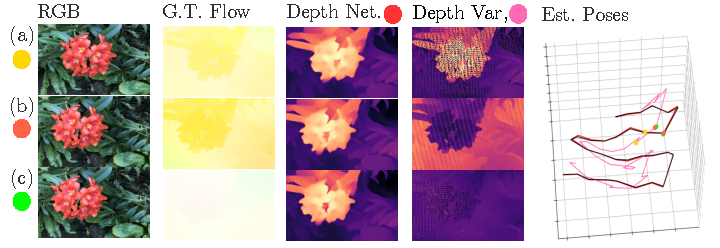
\includegraphics[width=\linewidth,]{figures/pdfs/patchmatch_full.pdf}
     \caption{\textbf{PatchMatch.} Frame (a) and (b) both contain geometry-informative flow, but due to the ambiguity of optical flow relating depth and speed of motion, different frames in the depth-variable optimization converge to different solutions; using a depth CNN yields a consistent solution to this ambiguity across frames. And in the case of small or rotation-dominant motion (c), the flow does not sufficiently inform geometry and the optimized depth is mostly planar.}
  \label{fig:patchmatch}
\end{figure*}


\subsection{Additional Point Clouds and Qualitative Pose Reconstructions}
In \cref{fig:add_clouds}, we display 12 additional point clouds plus estimated camera poses across popular datasets and scenes across the LLFF, Tanks and Temples, MipNeRF 360, and CO3D datasets.
FlowMap robustly recovers camera poses and scene geometry across these diverse, challenging, and real-world sequences.

\subsection{Failure Cases}
While running FlowMap, we observed failures on several scenes.
These include the Tanks-and-Temples Auditorium scene (our model struggles with rotation-dominant trajectories), the LLFF Leaves scene (our model falls into a ``hollow-face minimum''), and the Tanks-and-Temples Lighthouse scene (this video features a large lens flare which degrades the optical flow).
Future extensions to FlowMap could use an occlusion-aware formulation to avoid hollow-face minima.
